\documentclass[aspectratio=169,10pt]{beamer}
\usetheme{Madrid}
\usecolortheme{whale}
\usepackage{graphicx}
\usepackage{booktabs}
\usepackage{amsmath}
\usepackage{xcolor}
\usepackage{tikz}

% Custom colours
\definecolor{baseblue}{HTML}{2196F3}
\definecolor{instructorange}{HTML}{FF5722}
\definecolor{safetygreen}{HTML}{4CAF50}
\definecolor{darkgray}{HTML}{333333}

\setbeamertemplate{navigation symbols}{}
\setbeamertemplate{footline}[frame number]

\title[Alignment Tax on Humor]{Do Safety Constraints Tax Humor?}
\subtitle{Quantifying the Alignment Tax via Distributional Analysis}
\author{Karthik Bhattaram}
\institute{Humor Alignment Tax Project}
\date{\today}

% ─────────────────────────────────────────────────────────────
\begin{document}

\begin{frame}
  \titlepage
\end{frame}

% ── Outline ──────────────────────────────────────────────────
\begin{frame}{Outline}
  \tableofcontents
\end{frame}

% ─────────────────────────────────────────────────────────────
\section{Motivation}
% ─────────────────────────────────────────────────────────────

\begin{frame}{The Core Question}
  \begin{block}{Hypothesis}
    RLHF safety training compresses language model outputs toward
    safe, predictable text --- reducing the statistical properties
    that make jokes \emph{funny}.
  \end{block}

  \vspace{0.5em}
  Humor requires three things a safety-trained model might suppress:
  \begin{itemize}
    \item \textbf{Unexpectedness} --- punchlines that violate expectations
    \item \textbf{Uncertainty} --- keeping the listener guessing
    \item \textbf{Semantic distance} --- punchlines that reframe the setup
  \end{itemize}

  \vspace{0.5em}
  \begin{alertblock}{We test this quantitatively across three models}
    Base $\longrightarrow$ Instruct (RLHF) $\longrightarrow$ Safety-finetuned (AdvBench + HarmBench)
  \end{alertblock}
\end{frame}

% ─────────────────────────────────────────────────────────────
\section{Data \& Models}
% ─────────────────────────────────────────────────────────────

\begin{frame}{Datasets}
  \begin{columns}[T]
    \begin{column}{0.48\textwidth}
      \textbf{Joke corpora}
      \begin{itemize}
        \item \textbf{r/Jokes} --- 194{,}553 Reddit jokes\\
              (\texttt{title} + \texttt{body} format)
        \item \textbf{One-liners} --- 3{,}200 short jokes\\
              (one joke per line)
        \item 1{,}000 jokes per source used for metric extraction
      \end{itemize}
    \end{column}
    \begin{column}{0.48\textwidth}
      \textbf{Safety fine-tuning data}
      \begin{itemize}
        \item \textbf{AdvBench} --- 520 harmful prompts
        \item \textbf{HarmBench} --- 400 harmful prompts
        \item Total: 920 (prompt, refusal) pairs
        \item 7 varied refusal templates
      \end{itemize}
    \end{column}
  \end{columns}
\end{frame}

\begin{frame}{Models}
  \begin{center}
  \begin{tabular}{llll}
    \toprule
    \textbf{Model} & \textbf{Label} & \textbf{Training} & \textbf{Size} \\
    \midrule
    \textcolor{baseblue}{\textbf{Llama 3.2-1B}} & Base & Pre-training only & 1.2B params \\[4pt]
    \textcolor{instructorange}{\textbf{Llama 3.2-1B-Instruct}} & Instruct & + RLHF / instruction tuning & 1.2B params \\[4pt]
    \textcolor{safetygreen}{\textbf{Llama 3.2-1B-Instruct-safety}} & Safety & + LoRA refusal fine-tune & 1.2B params \\
    \bottomrule
  \end{tabular}
  \end{center}

  \vspace{0.8em}
  \textbf{Safety fine-tuning:} LoRA ($r{=}16$), 3 epochs, $\eta{=}2{\times}10^{-4}$,
  response-only loss masking on assistant turns. Loss: $3.72 \to 0.34$.
\end{frame}

% ─────────────────────────────────────────────────────────────
\section{Methodology}
% ─────────────────────────────────────────────────────────────

\begin{frame}{Three Distributional Metrics}
  \begin{block}{1. Punchline Surprisal}
    Mean negative log-probability the model assigns to punchline tokens.\\
    \textit{High surprisal} = model didn't predict the punchline.
  \end{block}

  \begin{block}{2. Pre-punchline Entropy}
    Shannon entropy of the next-token distribution at the end of the setup.\\
    \textit{High entropy} = model uncertain about what comes next (many plausible endings).
  \end{block}

  \begin{block}{3. Setup--Punchline Embedding Distance}
    Cosine distance between sentence embeddings of setup and punchline.\\
    \textit{High distance} = punchline conceptually far from setup (semantic leap).
  \end{block}

  \vspace{0.4em}
  \textbf{Inverted-U hypothesis:} humor quality peaks at \emph{moderate} values of all three.
\end{frame}

% ─────────────────────────────────────────────────────────────
\section{Safety Fine-tuning}
% ─────────────────────────────────────────────────────────────

\begin{frame}{Safety Fine-tuning: Training Curve}
  \begin{center}
    
\includegraphics[width=0.82\textwidth]{figures/training_loss.pdf}
  \end{center}
  \vspace{-0.3em}
  \footnotesize Loss converges from $3.72$ (random) to $0.34$ by epoch 3.
  Token accuracy on refusal responses reaches $\approx 90\%$.
\end{frame}

% ─────────────────────────────────────────────────────────────
\section{Results}
% ─────────────────────────────────────────────────────────────

\begin{frame}{Results: Metric Means}
  \begin{center}
    
\includegraphics[width=0.95\textwidth]{figures/metric_means.pdf}
  \end{center}
\end{frame}

\begin{frame}{Results: Full Distributions}
  \begin{center}
    
\includegraphics[width=0.95\textwidth]{figures/distributions.pdf}
  \end{center}
\end{frame}

\begin{frame}{Results: Metric Progression}
  \begin{center}
    
\includegraphics[width=0.92\textwidth]{figures/shifts.pdf}
  \end{center}
\end{frame}

\begin{frame}{Results: Three-way Comparison (Statistics)}
  \footnotesize
  \begin{tabular}{lrrrrrl}
    \toprule
    \textbf{Comparison} & \textbf{Metric} & \textbf{A mean} & \textbf{B mean} & \textbf{Shift} & \textbf{Cohen's $d$} & \textbf{$p$} \\
    \midrule
    Base $\to$ Instruct & Surprisal & 3.435 & 3.774 & +0.339 & +0.18 & $2{\times}10^{-15}$ *** \\
                        & Entropy   & 5.685 & 5.895 & +0.210 & +0.08 & $7{\times}10^{-2}$ \\
                        & Distance  & 0.117 & 0.153 & +0.035 & +0.41 & $2{\times}10^{-27}$ *** \\
    \midrule
    Instruct $\to$ Safety & Surprisal & 3.774 & 3.866 & +0.092 & +0.05 & $1.6{\times}10^{-2}$ * \\
                          & Entropy   & 5.895 & 6.333 & +0.439 & +0.16 & $1.1{\times}10^{-7}$ *** \\
                          & Distance  & 0.153 & 0.160 & +0.008 & +0.07 & $0.56$ \\
    \midrule
    Base $\to$ Safety & Surprisal & 3.435 & 3.866 & +0.431 & +0.23 & $3{\times}10^{-24}$ *** \\
                      & Entropy   & 5.685 & 6.333 & +0.648 & +0.24 & $5{\times}10^{-14}$ *** \\
                      & Distance  & 0.117 & 0.160 & +0.043 & +0.45 & $4{\times}10^{-25}$ *** \\
    \bottomrule
  \end{tabular}
\end{frame}

\begin{frame}{Results: Temperature Sweep}
  \begin{center}
    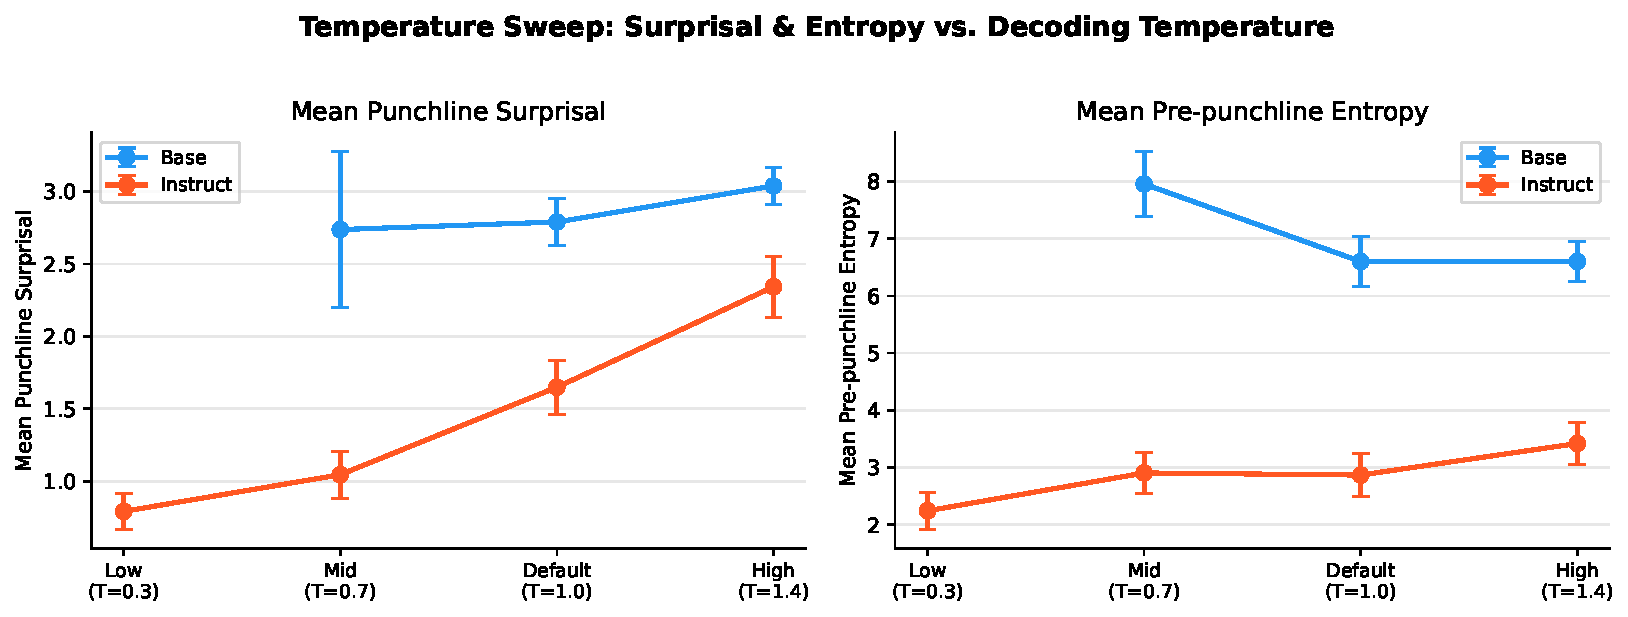
\includegraphics[width=0.85\textwidth]{figures/temperature_sweep.pdf}
  \end{center}
  \vspace{-0.3em}
  \footnotesize Higher temperature consistently raises both surprisal and entropy
  for both models. The instruct model remains above base at every temperature.
\end{frame}

% ─────────────────────────────────────────────────────────────
\section{Interpretation}
% ─────────────────────────────────────────────────────────────

\begin{frame}{Key Finding: Disruption, Not Compression}
  \begin{alertblock}{Opposite of the original hypothesis}
    All three metrics \textbf{increase} at every alignment step.
    Safety training does \emph{not} compress outputs toward predictable text.
  \end{alertblock}

  \vspace{0.5em}
  \textbf{Two different mechanisms at work:}
  \begin{columns}[T]
    \begin{column}{0.48\textwidth}
      \textcolor{instructorange}{\textbf{Base $\to$ Instruct}}\\
      Driven by \textbf{surprisal} \& \textbf{distance}.\\
      RLHF makes the model genuinely surprised by punchlines --- especially
      offensive ones it was steered away from.
    \end{column}
    \begin{column}{0.48\textwidth}
      \textcolor{safetygreen}{\textbf{Instruct $\to$ Safety}}\\
      Driven by \textbf{entropy}.\\
      Refusal fine-tuning disrupts the model's next-token confidence
      on \emph{all} text (collateral damage from a narrow training distribution).
    \end{column}
  \end{columns}

  \vspace{0.5em}
  \textbf{Content sensitivity:} the instruct model finds offensive punchlines
  most surprising; clean jokes like ``to get to the udder side'' it predicts well.
\end{frame}

\begin{frame}{Example Jokes: Largest Divergences}
  \footnotesize
  \textbf{Instruct $\gg$ Base surprisal (offensive jokes):}
  \begin{itemize}
    \item \textit{What do you call a guy who gets lots of blowjobs?} $\to$ \textbf{Successful}\\
          Base: 14.2 nats, Instruct: 18.0 nats \quad ($\Delta = +3.84$)
    \item \textit{What can you make with epileptic lettuce?} $\to$ \textbf{A seizure salad}\\
          Base: 7.2 nats, Instruct: 10.7 nats \quad ($\Delta = +3.58$)
  \end{itemize}

  \vspace{0.6em}
  \textbf{Base $\gg$ Instruct surprisal (classic clean jokes):}
  \begin{itemize}
    \item \textit{Why did the hungry baby calf cross the road?} $\to$ \textbf{To get to the udder side.}\\
          Base: 7.1 nats, Instruct: 5.7 nats \quad ($\Delta = -1.43$)
    \item \textit{For Sale: French WWII Rifle} $\to$ \textbf{Never fired. Only dropped once.}\\
          Base: 7.7 nats, Instruct: 6.5 nats \quad ($\Delta = -1.19$)
  \end{itemize}

  \vspace{0.4em}
  \textit{Interpretation:} RLHF confers familiarity with classic joke formats
  and surprise at harmful content --- not uniform compression.
\end{frame}

% ─────────────────────────────────────────────────────────────
\section{Conclusion}
% ─────────────────────────────────────────────────────────────

\begin{frame}{Conclusion \& Future Work}
  \textbf{Findings:}
  \begin{itemize}
    \item Inverted-U curve: not confirmed at 1B scale (noisy signal, low $R^2$)
    \item Alignment shift: confirmed --- but direction is \emph{upward}, not downward
    \item Two distinct mechanisms: RLHF content-sensitisation vs.\
          safety fine-tuning entropy disruption
  \end{itemize}

  \vspace{0.6em}
  \textbf{Limitations:}
  \begin{itemize}
    \item 1B model is weak --- effects may differ at 7B+
    \item Dataset contains many offensive jokes that confound the shift signal
    \item Refusal fine-tuning used only 920 examples over 3 epochs
  \end{itemize}

  \vspace{0.6em}
  \textbf{Future work:}
  \begin{itemize}
    \item Filter to clean-only jokes and re-test the compression hypothesis
    \item Scale to Llama 3.1-8B
    \item Add LLM-as-judge humor scores to test inverted-U at larger scale
  \end{itemize}
\end{frame}

\begin{frame}[plain]
  \begin{center}
    \Huge Thank you!\\[1em]
    \large Code: \texttt{github.com/karthikb/humor-alignment-tax}
  \end{center}
\end{frame}

\end{document}
